\chapter{RESULTS}

\section{{\bf{Findings}}}
{\bf In this chapter, we present the results and visualization of the data set and theory described in CHAPTER-2 and finally discuss the results.
}

\section{\bf EDA}
\subsection{Non - Graphical}
Based on summary statistics, there were found columns that had no variance. As such, those columns were removed from the dataset as per the reasoning in 2.3.1 Uni-variate.\\ 

\begin{figure}[htpb]
	\centering
	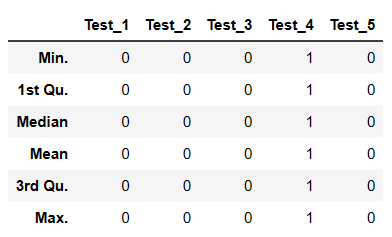
\includegraphics[height=10cm, width=12cm]{figures/s_stat.png}
	\caption{Columns With No Variance}
	\label{fig:columns}
\end{figure}
\noindent
Further more, the following columns were removed based on the domain of study as these columns were deemed to be less significant for further studies of the data. These are:

\begin{table}[htpb]
	\caption{Names Of Discarded Columns}
	\centering
	\begin{tabular}{|c|c|c|}
		\hline
		Patient Id & Patient First Name & Family Name \\
		Father's name & Institute Name  & Location of Institute\\
		Parental consent & Place of birth & H O radiation exposure x.ray\\
		H O substance abuse & & \\
		\hline
	\end{tabular}
	\label{tabl:discarded}
\end{table}

\begin{figure}[htpb]
	\centering
	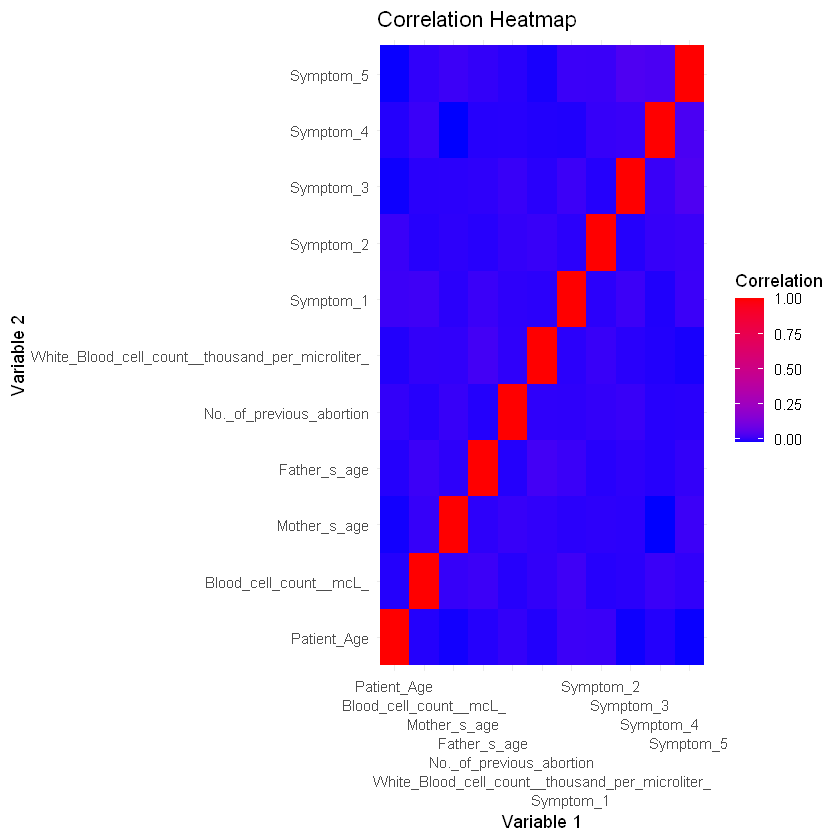
\includegraphics[height=10cm, width=12cm]{figures/corr.png}
	\caption{Correlation Heatmap Of Numeric Attributes}
	\label{fig 3}
\end{figure}

\noindent
Finally, the correlation between every pair of numeric attributes shows that there are no highly correlated attributes.

\newpage
\subsection{Graphical}
Based on the graphical analysis of the attributes in the dataset, we found many columns that does not provide any predictive value with regards to the target attributes.\\
\noindent
According to \cite{han2011data}, attribute significance is an important concept in data mining. The evaluation of attribute usefulness is crucial for effective data analysis. If the distribution of data across different attribute categories is equal, it indicates that the attribute does not have a strong discriminatory power to differentiate between the diseases. This lack of discriminatory power suggests that the attribute is not significantly associated with the diseases in the dataset.\\
\noindent
Similarly, \cite{mitchell1997machine} discusses the significance of attributes in machine learning. When the distribution of data is symmetric between different attribute categories, it implies that the attribute does not provide valuable predictive information for distinguishing between diseases. In this case, the symmetric distribution of data for the attribute suggests a lack of significance in relation to the diseases.\\

\begin{figure}[htpb]
	\centering
	\includegraphics[height=10cm, width=12cm]{figures/Status.png}
	\caption{Disorder And Status}
	\label{fig 4}
\end{figure}

\begin{figure}[htpb]
	\centering
	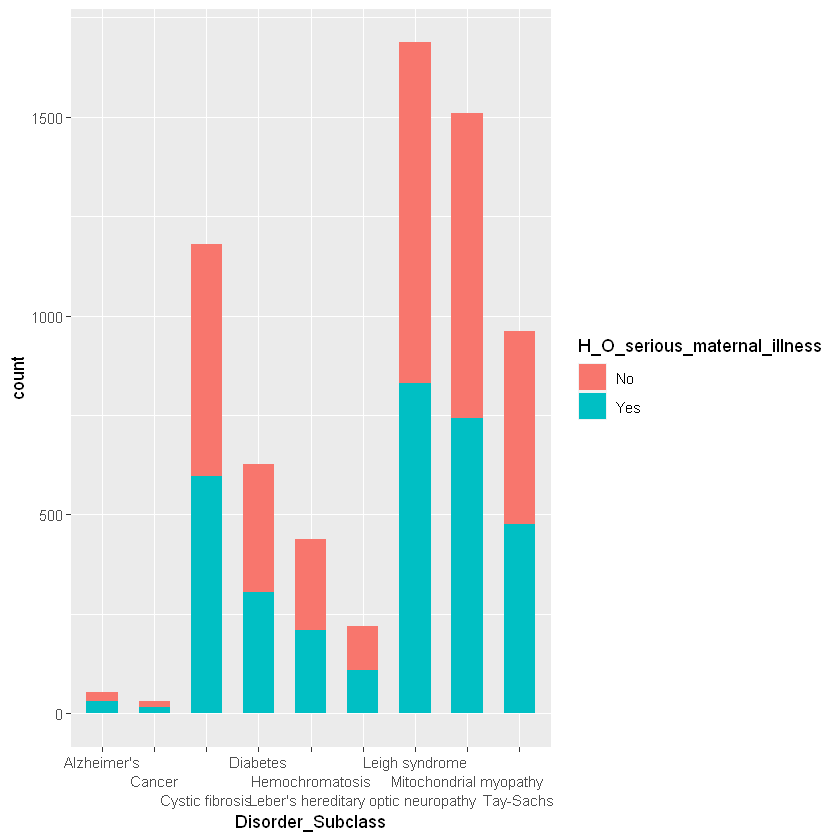
\includegraphics[height=10cm, width=12cm]{figures/maternalill.png}
	\caption{Disorder And History Of Maternal Illness}
	\label{fig 5}
\end{figure}

\begin{figure}[htpb]
	\centering
	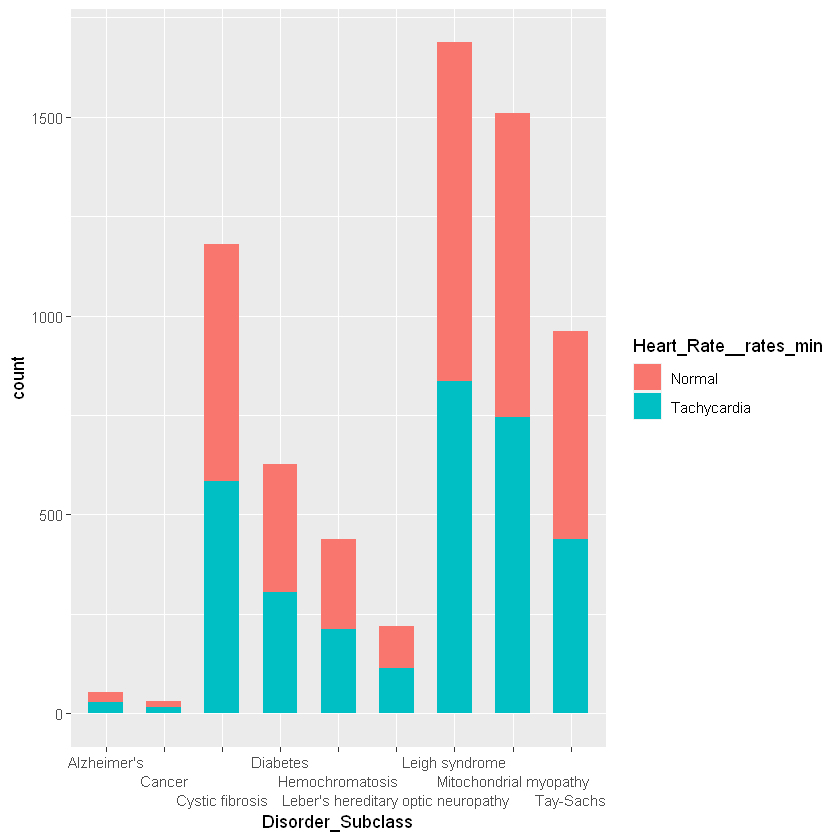
\includegraphics[height=10cm, width=12cm]{figures/heartrate.png}
	\caption{Disorder And Heart - rate}
	\label{fig 6}
\end{figure}

\begin{figure}[htpb]
	\centering
	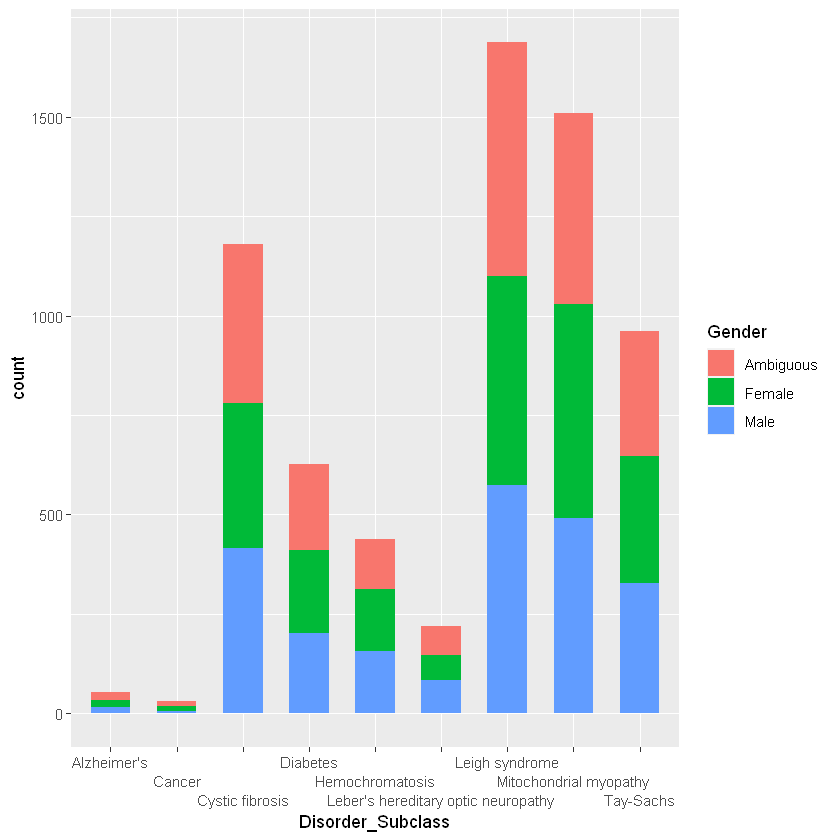
\includegraphics[height=10cm, width=12cm]{figures/gender.png}
	\caption{Disorder And Gender}
	\label{fig 7}
\end{figure}

\begin{figure}[htpb]
	\centering
	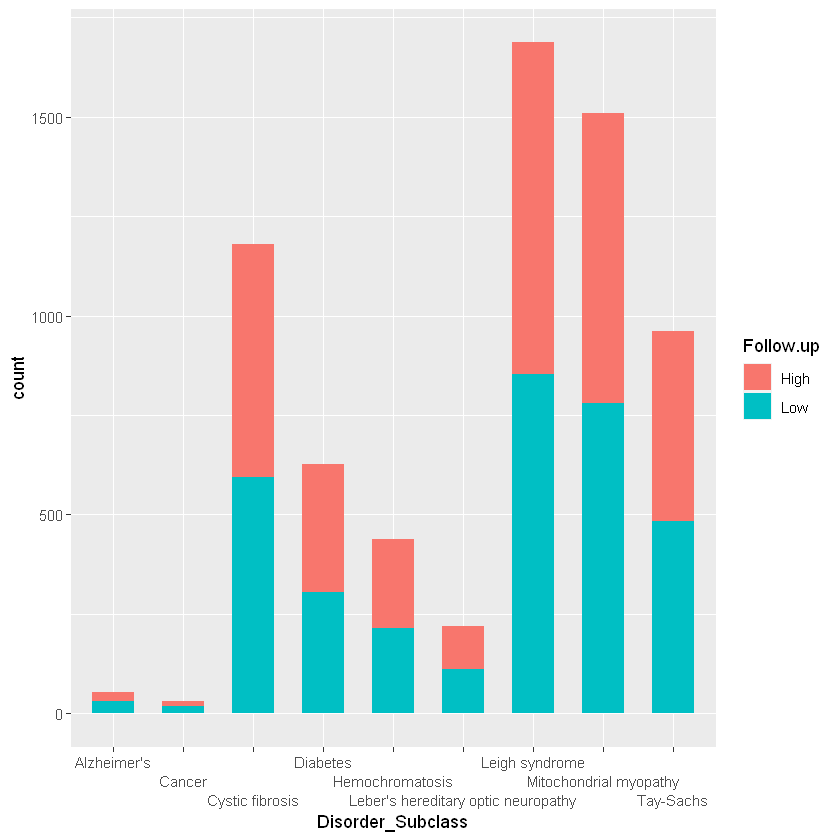
\includegraphics[height=10cm, width=12cm]{figures/follow.png}
	\caption{Disorder And Follow up}
	\label{fig 8}
\end{figure}

\begin{figure}[htpb]
	\centering
	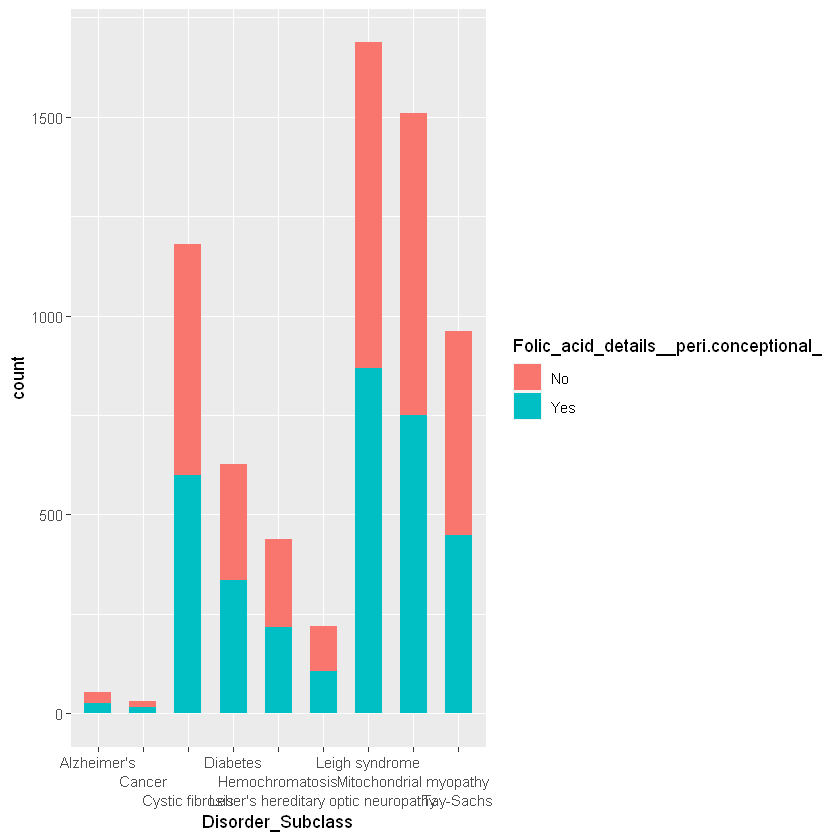
\includegraphics[height=10cm, width=12cm]{figures/folicacid.png}
	\caption{Disorder And Folic Acid details}
	\label{fig 9}
\end{figure}

\begin{figure}[htpb]
	\centering
	\includegraphics[height=10cm, width=12cm]{figures/Blood.png}
	\caption{Disorder And Blood Test Result}
	\label{fig 10}
\end{figure}

\begin{figure}[htpb]
	\centering
	\includegraphics[height=10cm, width=12cm]{figures/Birthdefect.png}
	\caption{Disorder And Birth Defect}
	\label{fig 11}
\end{figure}

\begin{figure}[htpb]
	\centering
	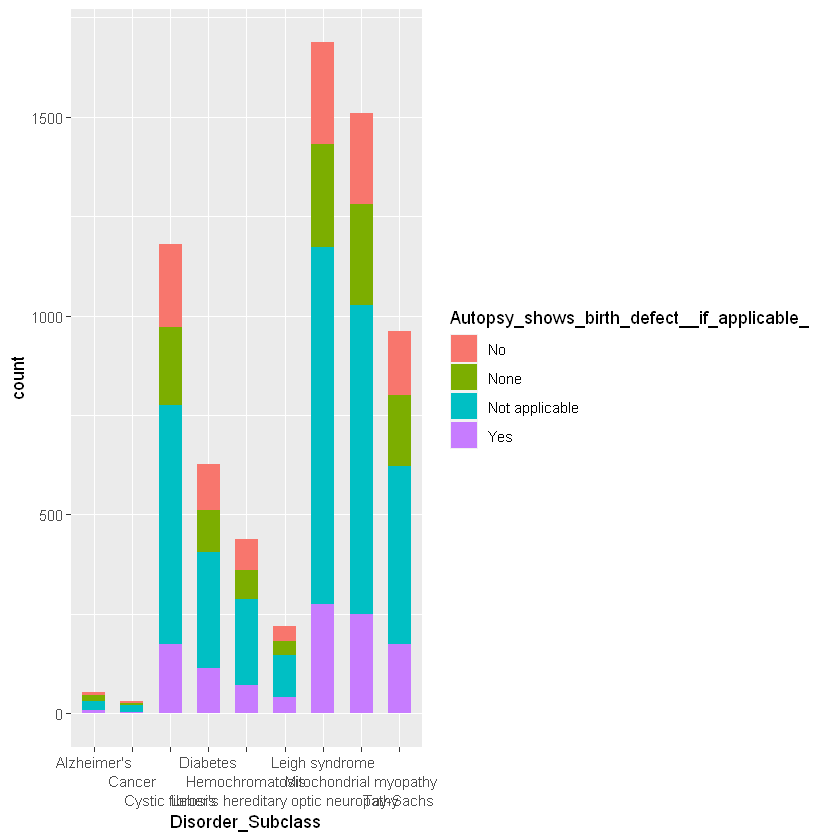
\includegraphics[height=10cm, width=12cm]{figures/autopsy.png}
	\caption{Disorder And Autopsy Report}
	\label{fig 12}
\end{figure}

\begin{figure}[htpb]
	\centering
	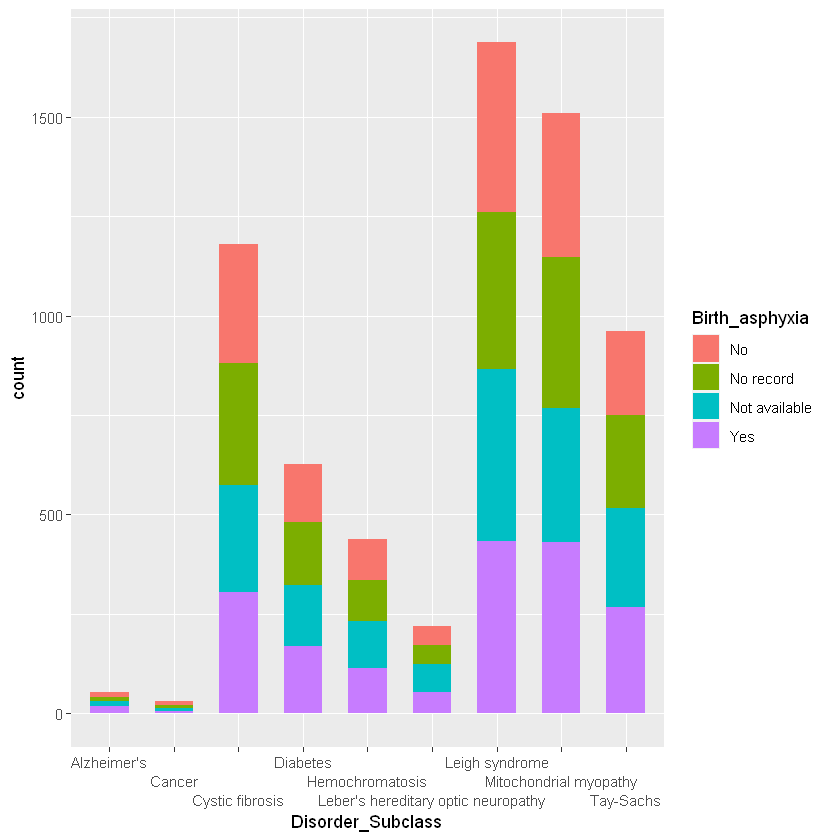
\includegraphics[height=10cm, width=12cm]{figures/asphyxia.png}
	\caption{Disorder And Asphyxia}
	\label{fig 13}
\end{figure}

\begin{figure}[htpb]
	\centering
	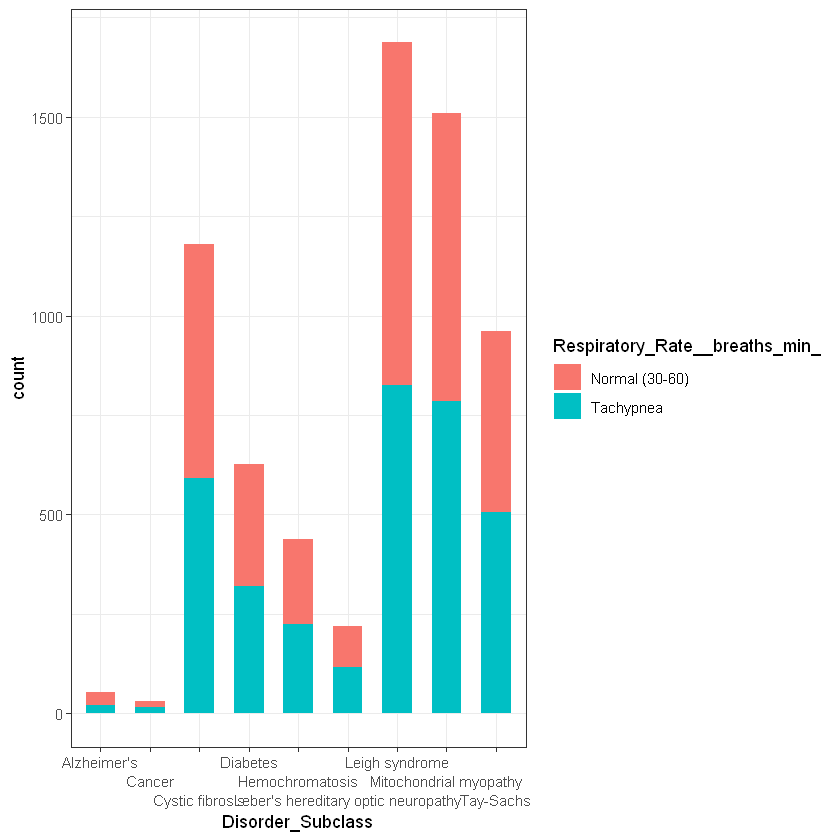
\includegraphics[height=10cm, width=12cm]{figures/resp.png}
	\caption{Disorder And Respiratory Rate}
	\label{fig 14}
\end{figure}

\begin{figure}[htpb]
	\centering
	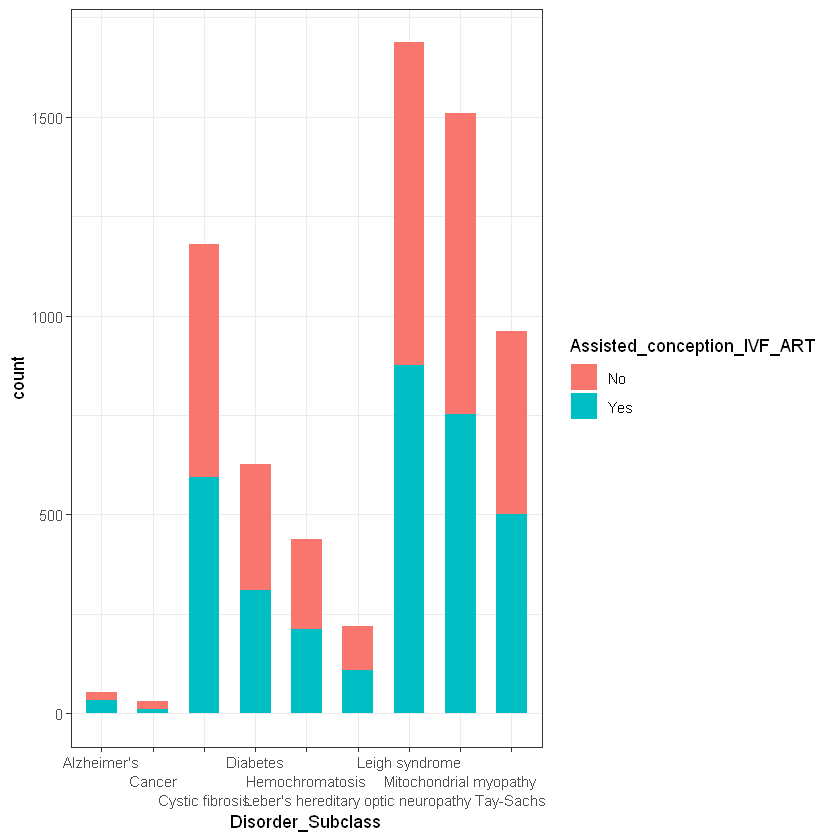
\includegraphics[height=10cm, width=12cm]{figures/ivf.png}
	\caption{Disorder And IVF details}
	\label{fig 15}
\end{figure}
\begin{figure}[htpb]
	\centering
	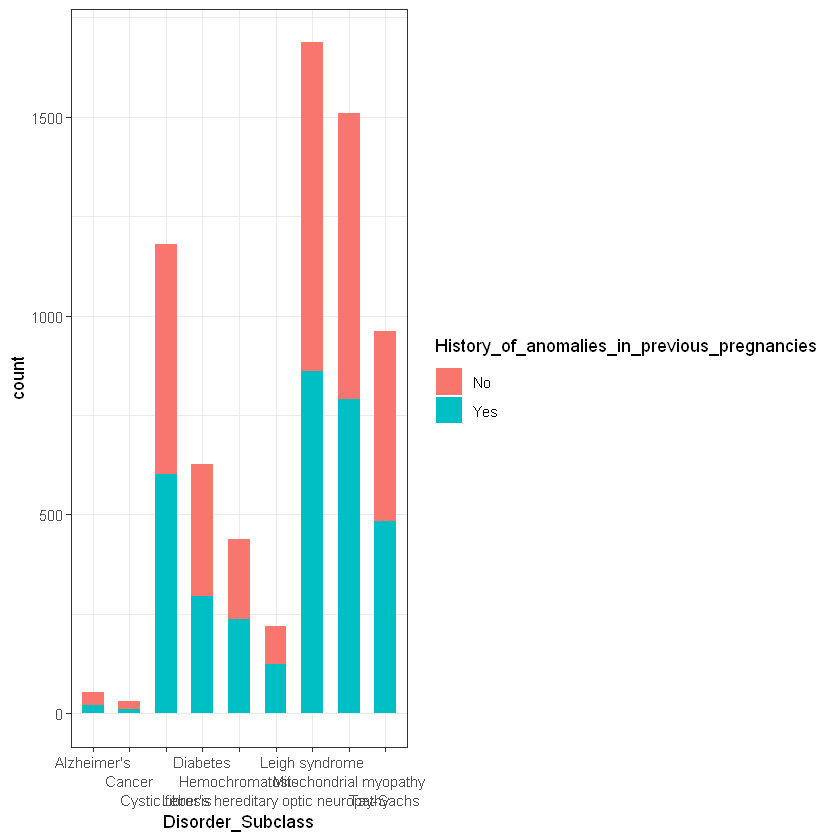
\includegraphics[height=10cm, width=12cm]{figures/preg.png}
	\caption{Disorder And History Of Pregnancy}
	\label{fig 16}
\end{figure}
\newpage
\noindent
We also found fully dependent relation between the two target attributes. That is, The Genetic Disorder attribute can be derived from the Disorder Subclass attribute. Hence that can also be now removed.
\begin{figure}[htpb]
	\centering
	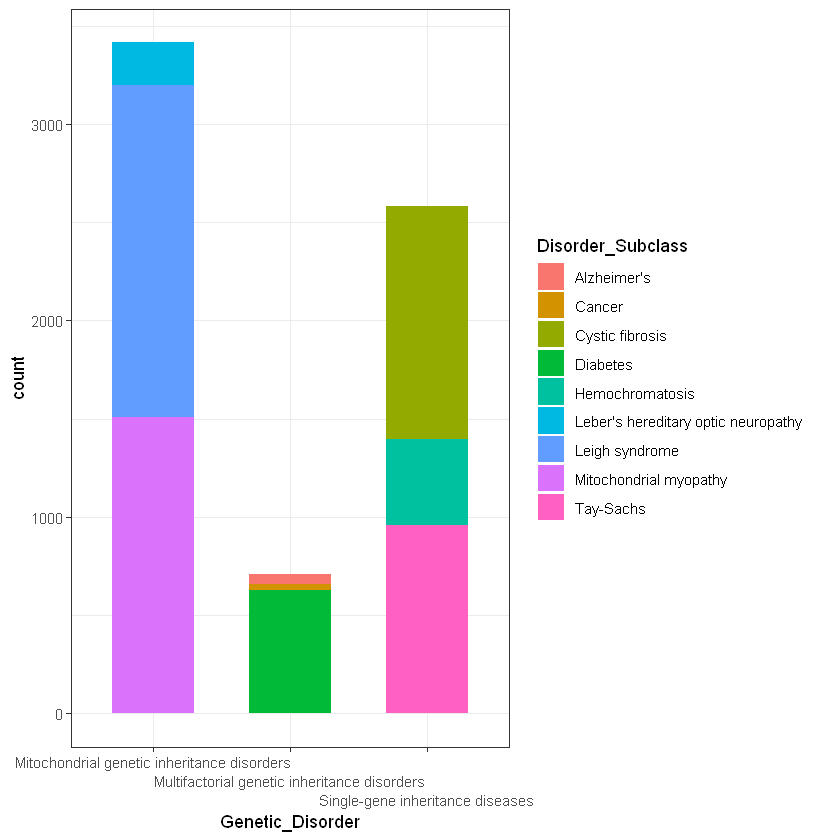
\includegraphics[height=10cm, width=12cm]{figures/rel.png}
	\caption{Relation Between Target Attributes }
	\label{fig 17}
\end{figure}
\paragraph{}

\noindent
\noindent
For the Numeric attributes, a disorder-wise Box and Whisker plots were created and it displayed relatively significant variance in one or more disorder.


\begin{figure}[htpb]
	\centering
	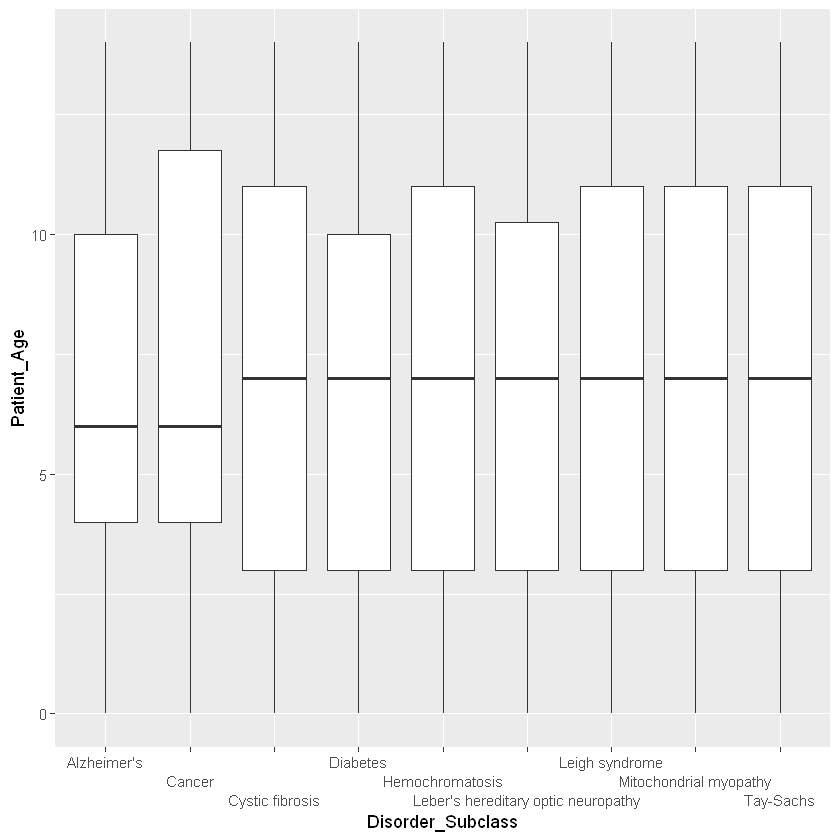
\includegraphics[height=10cm, width=12cm]{figures/p-age.png}
	\caption{Disorder And Patient's Age}
	\label{fig 18}
\end{figure}

\begin{figure}[htpb]
	\centering
	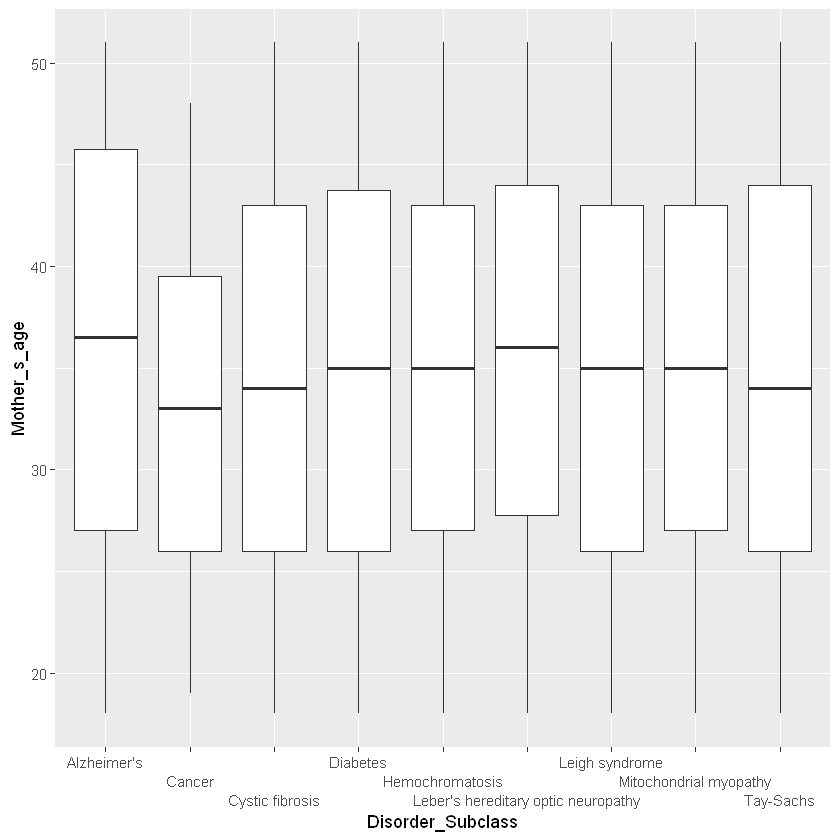
\includegraphics[height=10cm, width=12cm]{figures/m-age.png}
	\caption{Disorder And Patient's Mother's Age }
	\label{fig 19}
\end{figure}
\begin{figure}[htpb]
	\centering
	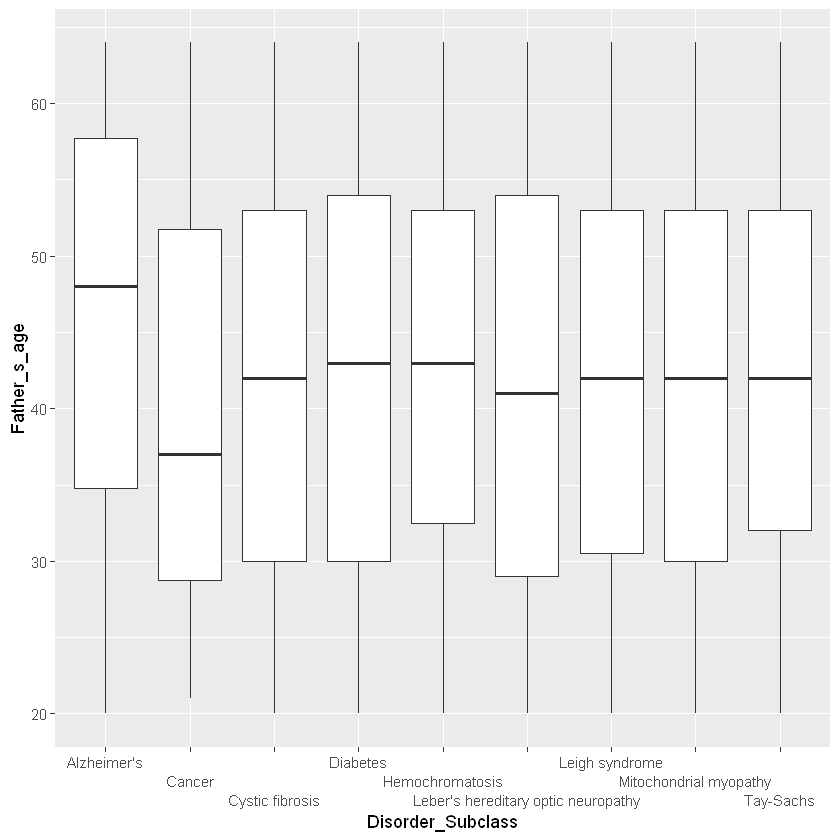
\includegraphics[height=10cm, width=12cm]{figures/f-age.png}
	\caption{Disorder And Patient's Father's Age }
	\label{fig 20}
\end{figure}
\begin{figure}[htpb]
	\centering
	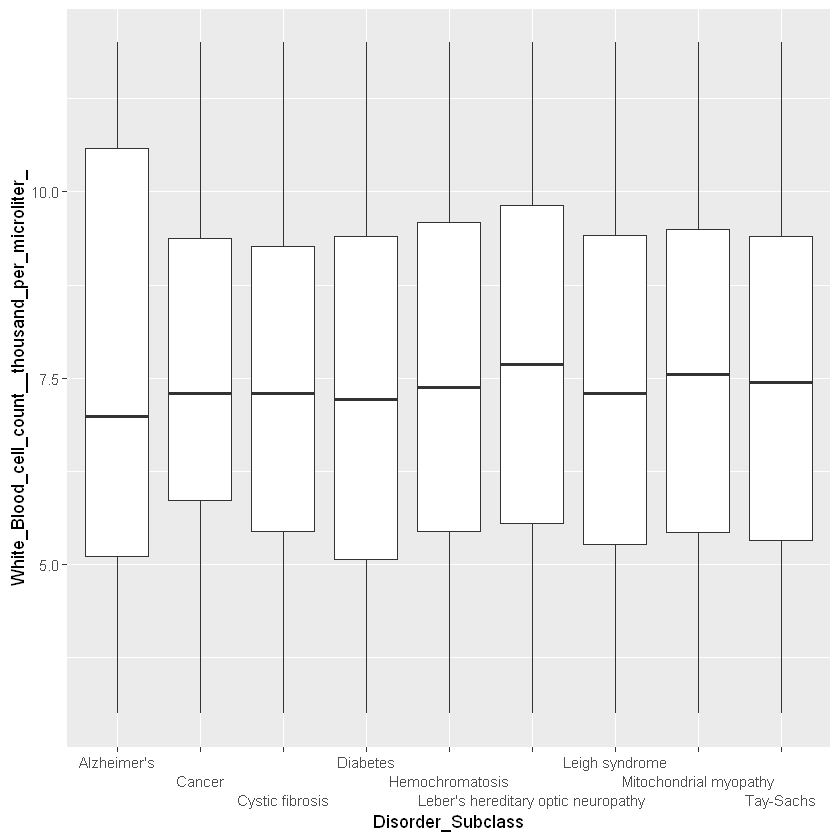
\includegraphics[height=10cm, width=12cm]{figures/wbc.png}
	\caption{Disorder And White Blood Cell Count}
	\label{fig 21}
\end{figure}
\begin{figure}[htpb]
	\centering
	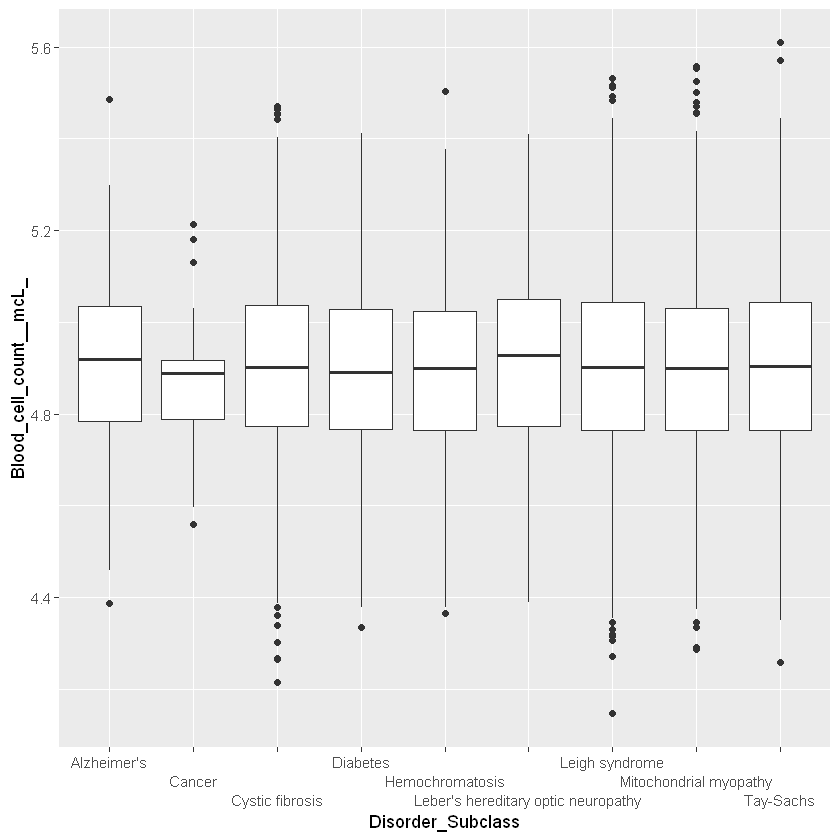
\includegraphics[height=10cm, width=12cm]{figures/bc.png}
	\caption{Disorder And Blood Cell Count}
	\label{fig 22}
\end{figure}
\begin{figure}[htpb]
	\centering
	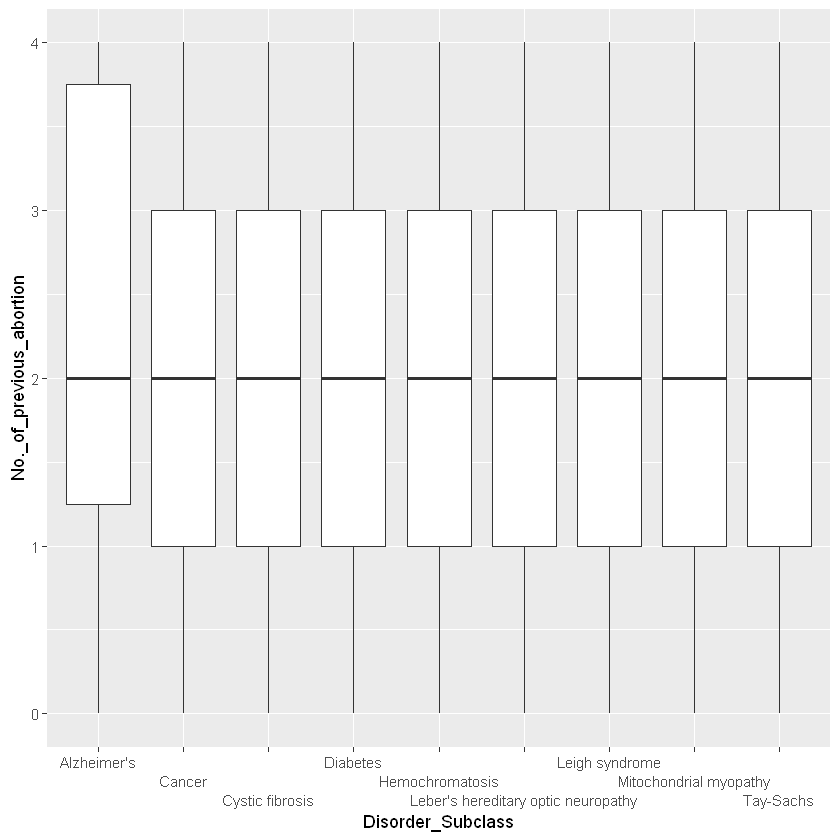
\includegraphics[height=10cm, width=12cm]{figures/npa.png}
	\caption{Disorder And Number Of Previous Abortions}
	\label{fig 23}
\end{figure}
\newpage
 \noindent
Based on the domain expertise the following columns are considered significant and have shown a good variance as such can prove proper information to classify the disorder on future data.
\begin{figure}[htpb]
	\centering
	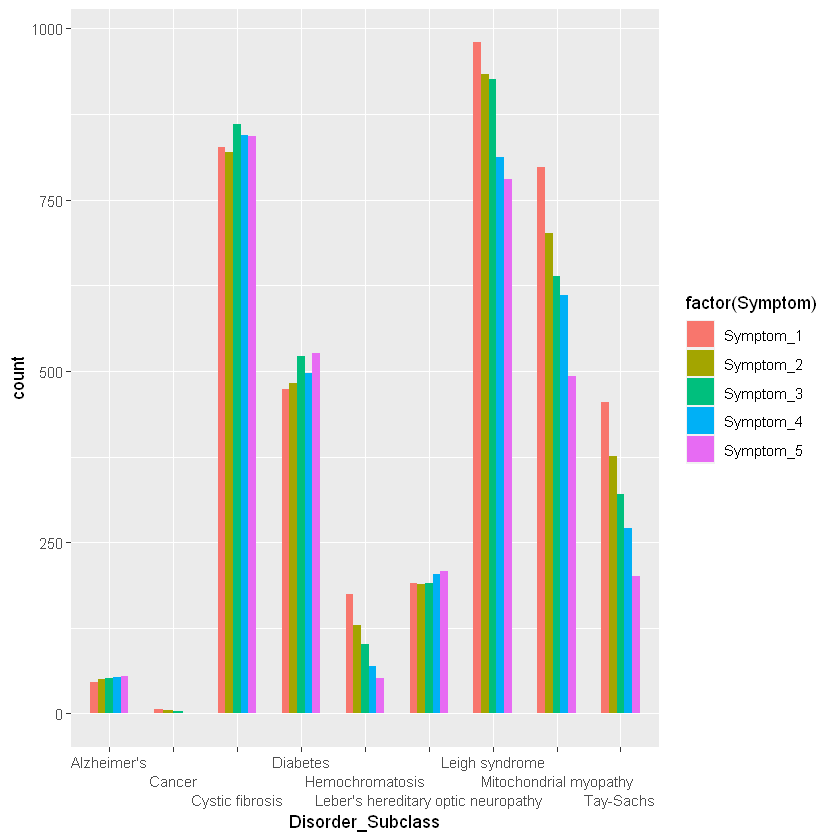
\includegraphics[height=8cm, width=10cm]{figures/s1.png}
	\caption{Disorder And Frequency Of Symptoms Being True}
	\label{fig 24}
\end{figure}
\begin{figure}[htpb]
	\centering
	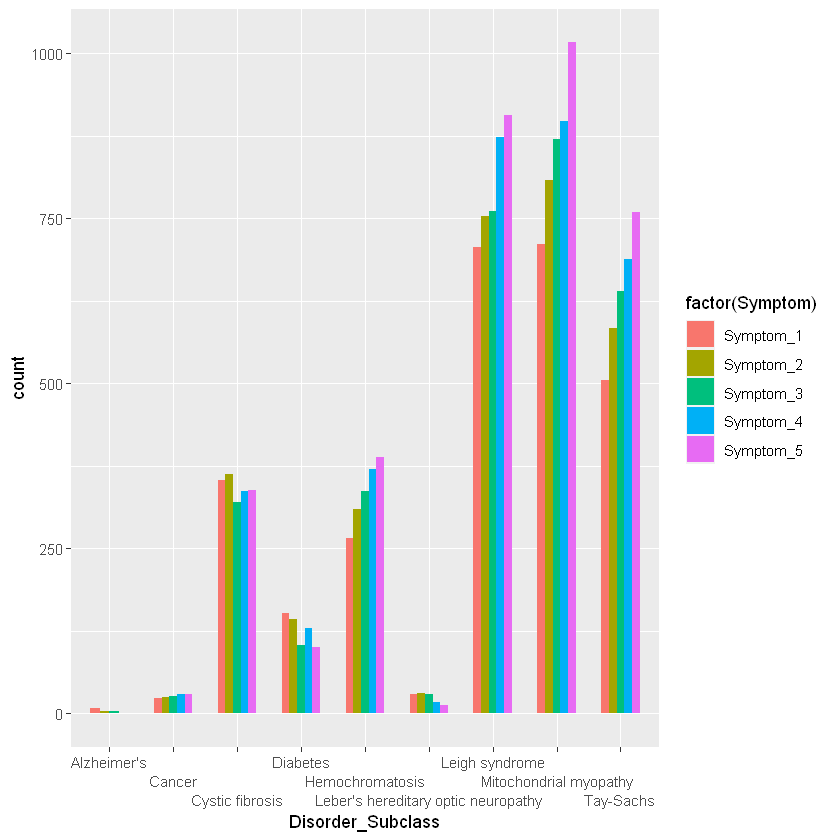
\includegraphics[height=8cm, width=10cm]{figures/s0.png}
	\caption{Disorder And Frequency Of Symptom Being False}
	\label{fig 25}
\end{figure}
\begin{figure}[htpb]
	\centering
	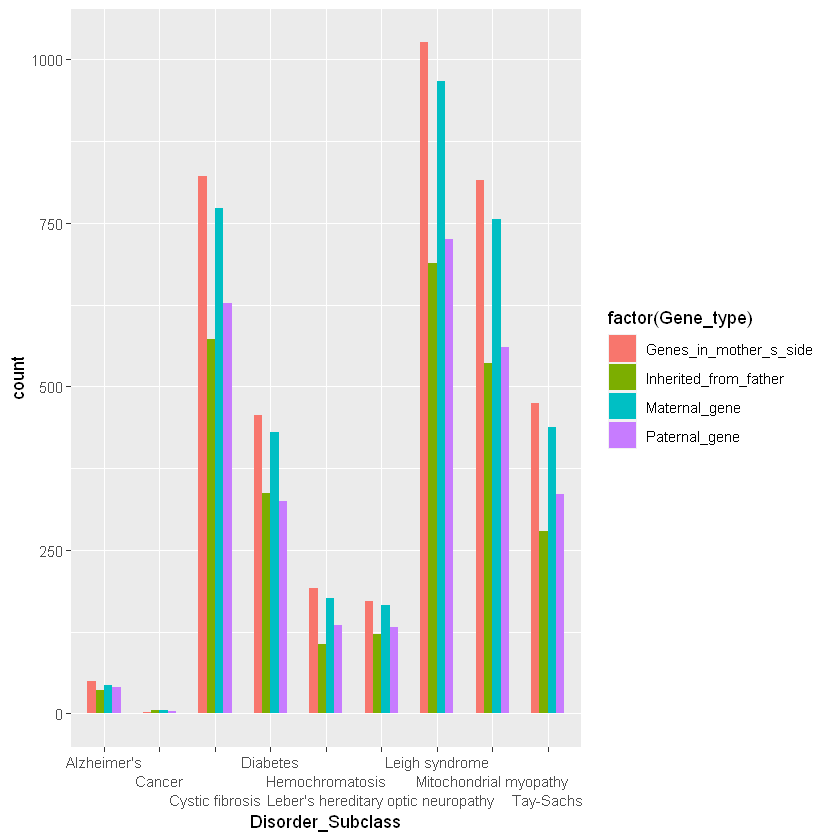
\includegraphics[height=10cm, width=12cm]{figures/gy.png}
	\caption{Disorder And Frequency Of Gene Being Yes}
	\label{fig 26}
\end{figure}
\begin{figure}[htpb]
	\centering
	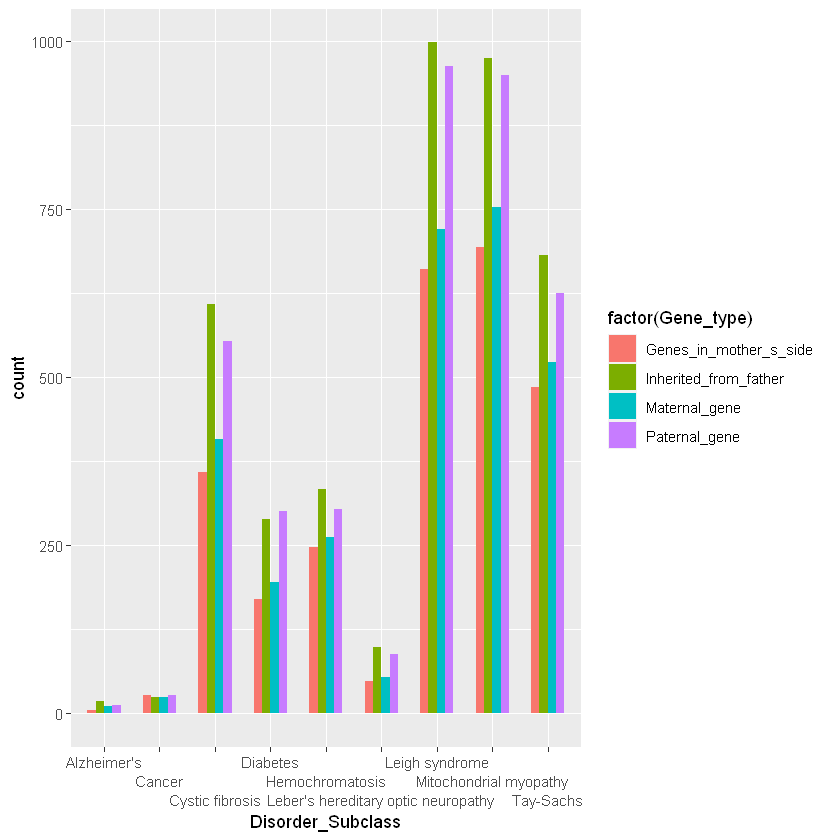
\includegraphics[height=10cm, width=12cm]{figures/gn.png}
	\caption{Disorder And Frequency Of Gene Being No}
	\label{fig 27}
\end{figure}
\newpage
\section{Dashboard}
Also an interactive dashboard is implemented using \url{https://visual.is} which can be found in \url{https://visual.is/visualizations/new-visualization/bpqD6MZM9CzQb8UTKZUThdx4}.\\
\begin{figure}[htpb]
	\centering
	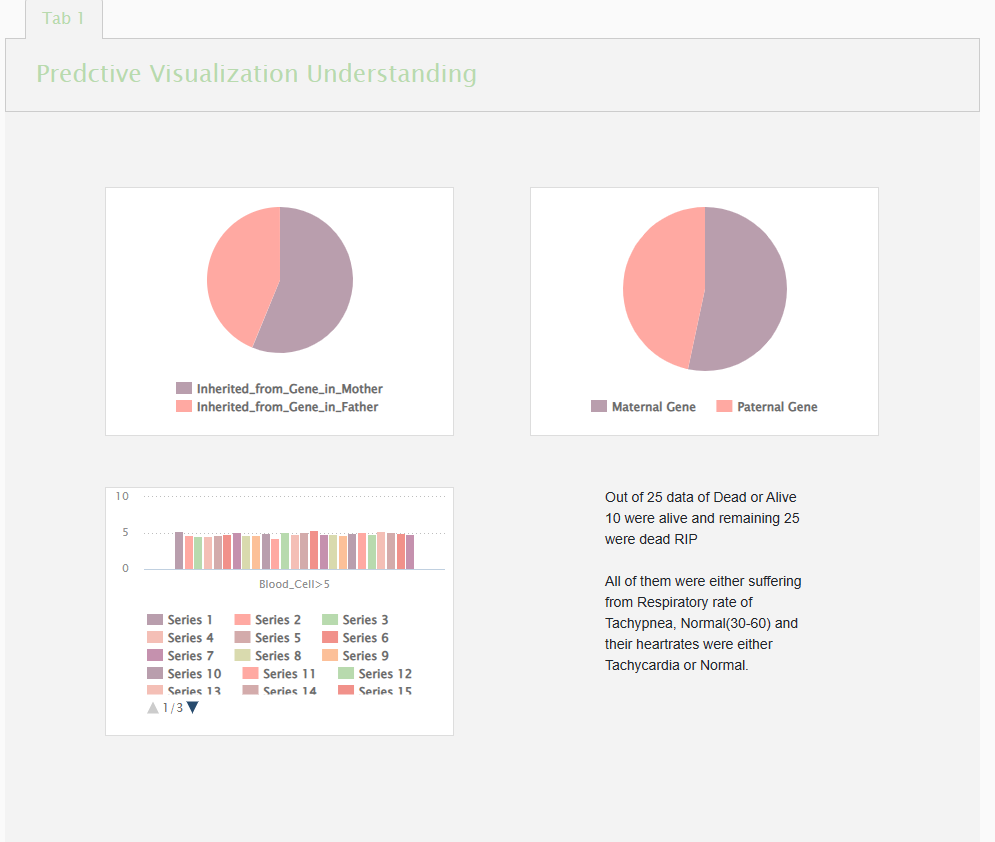
\includegraphics[height=10cm, width=12cm]{figures/dash.png}
	\caption{Dashboard Sample}
	\label{fig 28}
\end{figure}